\documentclass[conference]{IEEEtran}
%\IEEEoverridecommandlockouts
% The preceding line is only needed to identify funding in the first footnote. If that is unneeded, please comment it out.
\usepackage{cite}
\usepackage{amsmath,amssymb,amsfonts}
\usepackage{algorithmic}
\usepackage{graphicx}
\usepackage{textcomp}
\usepackage{xcolor}
\usepackage{float}
\def\BibTeX{{\rm B\kern-.05em{\sc i\kern-.025em b}\kern-.08em
    T\kern-.1667em\lower.7ex\hbox{E}\kern-.125emX}}
\graphicspath{{./Figures/}}    
    
    
    
\begin{document}

\title{Exploring the Role of Temporal Fine Structure and Envelope in Timbral Coding}

\author{\IEEEauthorblockN{Andrew Sivaprakasam}
\IEEEauthorblockA{\textit{Weldon School of Biomedical Engineering} \\
\textit{Purdue University}\\
West Lafayette, USA \\
asivapr@purdue.edu}}

\maketitle

\begin{abstract}
While the neural response to simple, stationary, and periodic auditory signals can be fairly well investigated, responses to auditory stimuli that are more complex, such as speech and music, are less well-characterized. Particularly, music is psychoacoustically complex. It is not well-understood how humans perceive the nuances of music, and how hearing impairment may affect the perception of such nuances. Before we can fully understand perception, we must first investigate how musical attributes like timbre are coded by the auditory periphery. By using a simulated auditory nerve model and comparing neural responses to stimulus envelope (ENV) and temporal fine structure (TFS), it is possible to see how timbral coding might be affected by hearing impairment. In this project, both instrumental timbre and articulation timbre were considered, and variations in coherence spectra of neural responses and Hilbert TFS/ENV were observed across instruments, articulations, and hearing impairment conditions.
\end{abstract}\vspace{1em}

\begin{IEEEkeywords}
auditory, neuroscience, music, modeling, envelope, temporal fine structure, timbre
\end{IEEEkeywords}

\section{Introduction}
The field of auditory neuroscience has made leaps and bounds in understanding how we percieve and code sounds that reach the cochlea. However, despite much study of perception of speech intelligibility and discrimination, the perception and coding of  \textit{music} still is quite under-investigated and remains an enigma. Though many auditory neuroscientists are musically inclined, music is quite complicated to study. Music is non-periodic and spectrally complicated. In the real-world setting, music is complex. Whether it be a symphony, rock concert, or music festival the soundstage varies, as does the articulation and instrumentation of the music itself, which makes it especially difficult to come up with a general set of rules or ideas that govern the way we hear and appreciate music. Additionally, psychoacoustics and musical training play a strong role in hearing \cite{bidelman_enhanced_2011}. Therefore, it is important to consider the differences in neural coding and perception that exist between varying instrumentation and articulation.

One way of assessing these difference is investigating the \textit{timbre} and how we respond to sounds of varying timbre. Timbre is the complex psychoacoustic phenomenon that allows us to discriminate between different ``colors" or ``qualities" of music. It is also the phenomenon that allows us to know when the same pitch is played by a different instrument. Though the perception of timbre is likely dependent on perception and musical training, there is no doubt that physical properties of timbre and the coding of these features are important, as well. In fact, recent work shows that normal hearing subjects rely on temporal fine structure to differentiate between instruments, while cochlear implant users rely almost exclusively on the envelope \cite{heng_impaired_2011}. But the question remains, \textit{what features of timbral coding are most relevant, and are these features impacted by hearing loss?} Answering this question could lead to innovations in hearing-assistive technology to improve the representation of music in devices such as cochlear implants and hearing aids.

\begin{figure}
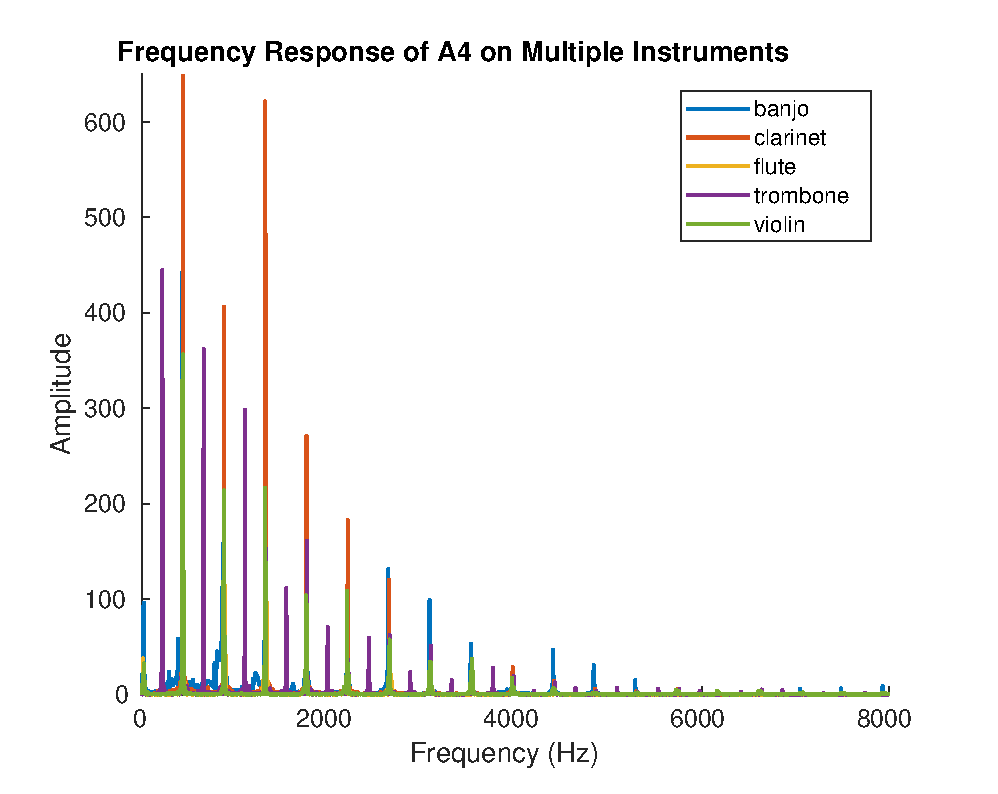
\includegraphics[width = .5\textwidth]{fft_all}
\caption{Spectra of five different instruments playing an A4 (440 Hz) tone. Variations in harmonic magnitude between instruments play a role in their characteristic sounds.}
\label{fig:fft_all}
\end{figure}

\begin{figure}[h!]
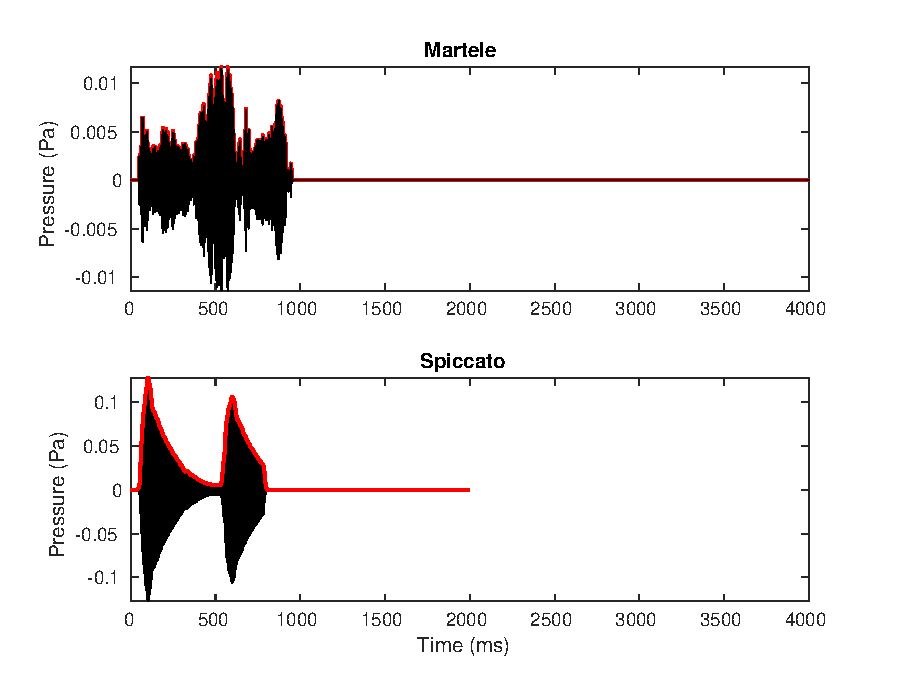
\includegraphics[width = .5\textwidth]{martele_spiccato_compare}
\caption{Variations in envelope (\textcolor{red}{red}) for two different articulations played by the violin. Waveforms were gammatone-filtered with a central frequency of 440 Hz.}
\label{fig:articulation}
\end{figure}

\subsection{The Physics of Timbre}
Variations in spectrotemporal content between instruments and their articulations is a good first step in assessing the differences in timbre from instrument to instrument. Isolating the physical characteristics of a sound played by one instrument that makes it unique from another is a key step in being able to study the coding of those characteristics. 

Figure \ref{fig:fft_all} shows the variations in the magnitude of the harmonics present in the same A4 (440 Hz) tone played on five different instruments. These same harmonics are also very pronounced in the spectrograms illustrated in Figure \ref{fig:spects}. Though it is somewhat obvious that these harmonic differences alter the physics and fine structure of a musical note, it less known how important this fine structure is in driving the coding and perception of that note by the auditory system.



The envelope of a tone also varies from instrument to instrument. Changes in envelope, even within a single instrument, can be observed by playing different articulations of that instrument. Figure \ref{fig:articulation} demonstrates variations in the envelope between the two violin articulations \textit{martel\'{e}} and \textit{spiccato}. Martel\'{e} is a more ``hammered" style of bowing, while spiccato is more ``bouncy, light, and separate."

\begin{figure*}
\includegraphics[width = \textwidth]{spects}
\caption{Spectrograms of three different instruments playing A4. Differences in onset and decay characterstics, modulations, and harmonic content may be visualized. Interestingly, harmonics of A3 (220 Hz) were found in the trombone recording for A4, demonstrating that timbral features may not necessarily be limited to the harmonics of the fundamental frequency of the note being played.}
\label{fig:spects}
\end{figure*}


\subsection{Methods of Analysis for Investigating TFS and ENV Neural Responses}
Much progress has been made on developing methods and analyses by which we can study how features of a particular sound stimulus reach the auditory nerve, and how they may be processed by higher order systems within the brain and brainstem. Particularly, the envelope (ENV) and temporal fine structure (TFS) of a given stimulus have been established as having relevance in its perception \cite{smith_chimaeric_2002}. However, \textit{perception }is different from \textit{coding}, and further signal processing methods were designed to characterize how TFS and ENV features are encoded by the auditory nerve \cite{heinz_quantifying_2009}. More recently, Parida et al. have developed a spectrally-specific framework for investigating ENV and TFS that can be applied to spike trains \textit{and} non-invasive far-field measures like frequency following responses (FFRs) \cite{parida_spectrally_2020}. This framework can also be applied to non-stationary signals. 

\subsection{Modeling the Auditory Nerve} 

To record neural spike data at the level of the auditory nerve is an acute and invasive process. Each experiment may span several hours, or even days.  Therefore, being sure that the stimulus presentation and signal acquistion match the question being investigated is important. One way to reduce the time needed to get data and animals needed for experimentation is using an auditory nerve model.

Zilany et al. created the auditory nerve model that was last updated in 2018, BEZ2018 \cite{bruce_phenomenological_2018}. This model is highly regarded by the field of auditory neuroscience. Though there is no replacement for true electrophysiological data, it is helpful to have an \textit{in silico} model with customizable parameters that may guide \textit{in vivo} experimentation in the future. At the very least, it allows researchers to test the validity of spike train analysis so that when \textit{in vivo} experiments may be conducted, the analysis is refined enough to answer the question at hand.
 
\subsection{A Generalizable Framework for Studying Timbre} 
 
While studies have investigated timbral \textit{perception} and have even proposed means of quantifying this perceptual ability, we are not aware of any studies that have investigated timbral \textit{coding} \cite{lee_timbre_2020}. By combining the modeling work from Zilany et al. and the spectrally specific framework designed by Parida et al., a new framework for analysis can be created to study ENV and TFS coding in various instrumental sounds and how they may or may not be impacted by hearing loss. By using this framework to identify relevant timbral coding features \textit{in silico}, recommendations for future \textit{in vivo} timbral coding experiments can be suggested. Additionally, the spectral analysis methods outlined in this new framework can be applied to \textit{both} invasive auditory nerve experiments and non-invasive FFR experiments due to the generalizabilty of the methods developed by Parida et al.
 
\section{Methods}

A framework was developed to investigate timbral coding using a combination of auditory nerve modeling and application of a spectrally-specific framework to study the strength of ENV and TFS coding across various instruments and articulations. Figure \ref{fig:flow} represents a general flow diagram of the methods used.


\subsection{Sound Stimuli}

All sound stimuli were acquired from the Philharmonia Orchestra's (UK) sound sample database \cite{noauthor_sound_nodate}. This sound sample library has thousands of neatly categorized and concise recordings that span the instrumental range of the standard orchestra, over several pitches, articulations, and expressions. The sound samples were resampled in MATLAB (Natick, MA) to 100 kHz in order to be processed by the auditory nerve model. To assess timbral coding variations between instruments, banjo, clarinet, flute, trombone, and violin A4 (440 Hz) tones were used. To assess differences in timbral coding between articulation, a martel\'{e} and spiccato sound at A4 on the violin was used.  

\subsection{Auditory Nerve Model}
The BEZ2018 model was used to generate spike 


\subsection{Stimulus Filtering}

Stimuli were passed through a computationally efficient gammatone filterbank 





\subsection{Equations}
Number equations consecutively. To make your 
equations more compact, you may use the solidus (~/~), the exp function, or 
appropriate exponents. Italicize Roman symbols for quantities and variables, 
but not Greek symbols. Use a long dash rather than a hyphen for a minus 
sign. Punctuate equations with commas or periods when they are part of a 
sentence, as in:
\begin{equation}
a+b=\gamma\label{eq}
\end{equation}

Be sure that the 
symbols in your equation have been defined before or immediately following 
the equation. Use ``\eqref{eq}'', not ``Eq.~\eqref{eq}'' or ``equation \eqref{eq}'', except at 
the beginning of a sentence: ``Equation \eqref{eq} is . . .''

\subsection{\LaTeX-Specific Advice}

Please use ``soft'' (e.g., \verb|\eqref{Eq}|) cross references instead
of ``hard'' references (e.g., \verb|(1)|). That will make it possible
to combine sections, add equations, or change the order of figures or
citations without having to go through the file line by line.

Please don't use the \verb|{eqnarray}| equation environment. Use
\verb|{align}| or \verb|{IEEEeqnarray}| instead. The \verb|{eqnarray}|
environment leaves unsightly spaces around relation symbols.

Please note that the \verb|{subequations}| environment in {\LaTeX}
will increment the main equation counter even when there are no
equation numbers displayed. If you forget that, you might write an
article in which the equation numbers skip from (17) to (20), causing
the copy editors to wonder if you've discovered a new method of
counting.

{\BibTeX} does not work by magic. It doesn't get the bibliographic
data from thin air but from .bib files. If you use {\BibTeX} to produce a
bibliography you must send the .bib files. 

{\LaTeX} can't read your mind. If you assign the same label to a
subsubsection and a table, you might find that Table I has been cross
referenced as Table IV-B3. 

{\LaTeX} does not have precognitive abilities. If you put a
\verb|\label| command before the command that updates the counter it's
supposed to be using, the label will pick up the last counter to be
cross referenced instead. In particular, a \verb|\label| command
should not go before the caption of a figure or a table.

Do not use \verb|\nonumber| inside the \verb|{array}| environment. It
will not stop equation numbers inside \verb|{array}| (there won't be
any anyway) and it might stop a wanted equation number in the
surrounding equation.
\begin{figure*}
\includegraphics[width = \textwidth]{methods_flow_sanspic}
\caption{Methods flow diagram. Different instrument and articulation stimuli were processed through the BEZ2018 auditory nerve model  and through a gammatone filterbank. Alternating-polarity peristimulus time histograms (apPSTHs) (\textcolor{red}{red}) from the auditory nerve model were processed to extract TFS and ENV-related responses, and these were compared to the Hilbert TFS and ENV (\textcolor{blue}{blue}) extracted from the gammatone-filtered stimuli by means of Magnitude-Squared Coherence.}
\label{fig:flow}
\end{figure*}
\subsection{Some Common Mistakes}\label{SCM}
\begin{itemize}
\item The word ``data'' is plural, not singular.
\item The subscript for the permeability of vacuum $\mu_{0}$, and other common scientific constants, is zero with subscript formatting, not a lowercase letter ``o''.
\item In American English, commas, semicolons, periods, question and exclamation marks are located within quotation marks only when a complete thought or name is cited, such as a title or full quotation. When quotation marks are used, instead of a bold or italic typeface, to highlight a word or phrase, punctuation should appear outside of the quotation marks. A parenthetical phrase or statement at the end of a sentence is punctuated outside of the closing parenthesis (like this). (A parenthetical sentence is punctuated within the parentheses.)
\item A graph within a graph is an ``inset'', not an ``insert''. The word alternatively is preferred to the word ``alternately'' (unless you really mean something that alternates).
\item Do not use the word ``essentially'' to mean ``approximately'' or ``effectively''.
\item In your paper title, if the words ``that uses'' can accurately replace the word ``using'', capitalize the ``u''; if not, keep using lower-cased.
\item Be aware of the different meanings of the homophones ``affect'' and ``effect'', ``complement'' and ``compliment'', ``discreet'' and ``discrete'', ``principal'' and ``principle''.
\item Do not confuse ``imply'' and ``infer''.
\item The prefix ``non'' is not a word; it should be joined to the word it modifies, usually without a hyphen.
\item There is no period after the ``et'' in the Latin abbreviation ``et al.''.
\item The abbreviation ``i.e.'' means ``that is'', and the abbreviation ``e.g.'' means ``for example''.
\end{itemize}
An excellent style manual for science writers is \cite{b7}.

\subsection{Authors and Affiliations}
\textbf{The class file is designed for, but not limited to, six authors.} A 
minimum of one author is required for all conference articles. Author names 
should be listed starting from left to right and then moving down to the 
next line. This is the author sequence that will be used in future citations 
and by indexing services. Names should not be listed in columns nor group by 
affiliation. Please keep your affiliations as succinct as possible (for 
example, do not differentiate among departments of the same organization).

\subsection{Identify the Headings}
Headings, or heads, are organizational devices that guide the reader through 
your paper. There are two types: component heads and text heads.

Component heads identify the different components of your paper and are not 
topically subordinate to each other. Examples include Acknowledgments and 
References and, for these, the correct style to use is ``Heading 5''. Use 
``figure caption'' for your Figure captions, and ``table head'' for your 
table title. Run-in heads, such as ``Abstract'', will require you to apply a 
style (in this case, italic) in addition to the style provided by the drop 
down menu to differentiate the head from the text.

Text heads organize the topics on a relational, hierarchical basis. For 
example, the paper title is the primary text head because all subsequent 
material relates and elaborates on this one topic. If there are two or more 
sub-topics, the next level head (uppercase Roman numerals) should be used 
and, conversely, if there are not at least two sub-topics, then no subheads 
should be introduced.

\subsection{Figures and Tables}
\paragraph{Positioning Figures and Tables} Place figures and tables at the top and 
bottom of columns. Avoid placing them in the middle of columns. Large 
figures and tables may span across both columns. Figure captions should be 
below the figures; table heads should appear above the tables. Insert 
figures and tables after they are cited in the text. Use the abbreviation 
``Fig.~\ref{fig}'', even at the beginning of a sentence.

%\begin{table}[htbp]
%\caption{Table Type Styles}
%\begin{center}
%\begin{tabular}{|c|c|c|c|}
%\hline
%\textbf{Table}&\multicolumn{3}{|c|}{\textbf{Table Column Head}} \\
%\cline{2-4} 
%\textbf{Head} & \textbf{\textit{Table column subhead}}& \textbf{\textit{Subhead}}& \textbf{\textit{Subhead}} \\
%\hline
%copy& More table copy$^{\mathrm{a}}$& &  \\
%\hline
%\multicolumn{4}{l}{$^{\mathrm{a}}$Sample of a Table footnote.}
%\end{tabular}
%\label{tab1}
%\end{center}
%\end{table}
%
%\begin{figure}[htbp]
%\centerline{\includegraphics{fig1.png}}
%\caption{Example of a figure caption.}
%\label{fig}
%\end{figure}

Figure Labels: Use 8 point Times New Roman for Figure labels. Use words 
rather than symbols or abbreviations when writing Figure axis labels to 
avoid confusing the reader. As an example, write the quantity 
``Magnetization'', or ``Magnetization, M'', not just ``M''. If including 
units in the label, present them within parentheses. Do not label axes only 
with units. In the example, write ``Magnetization (A/m)'' or ``Magnetization 
\{A[m(1)]\}'', not just ``A/m''. Do not label axes with a ratio of 
quantities and units. For example, write ``Temperature (K)'', not 
``Temperature/K''.

\section*{Acknowledgment}

The preferred spelling of the word ``acknowledgment'' in America is without 
an ``e'' after the ``g''. Avoid the stilted expression ``one of us (R. B. 
G.) thanks $\ldots$''. Instead, try ``R. B. G. thanks$\ldots$''. Put sponsor 
acknowledgments in the unnumbered footnote on the first page.

\section*{References}

Please number citations consecutively within brackets \cite{b1}. The 
sentence punctuation follows the bracket \cite{b2}. Refer simply to the reference 
number, as in \cite{b3}---do not use ``Ref. \cite{b3}'' or ``reference \cite{b3}'' except at 
the beginning of a sentence: ``Reference \cite{b3} was the first $\ldots$''

Number footnotes separately in superscripts. Place the actual footnote at 
the bottom of the column in which it was cited. Do not put footnotes in the 
abstract or reference list. Use letters for table footnotes.

Unless there are six authors or more give all authors' names; do not use 
``et al.''. Papers that have not been published, even if they have been 
submitted for publication, should be cited as ``unpublished'' \cite{b4}. Papers 
that have been accepted for publication should be cited as ``in press'' \cite{b5}. 
Capitalize only the first word in a paper title, except for proper nouns and 
element symbols.

For papers published in translation journals, please give the English 
citation first, followed by the original foreign-language citation \cite{b6}.

\bibliographystyle{ieeetr}
%laptop
%\bibliographystyle{IEEEtran} 

\bibliography{references}{}

\end{document}
